\chapter{Joshua 10}

\begin{figure}
  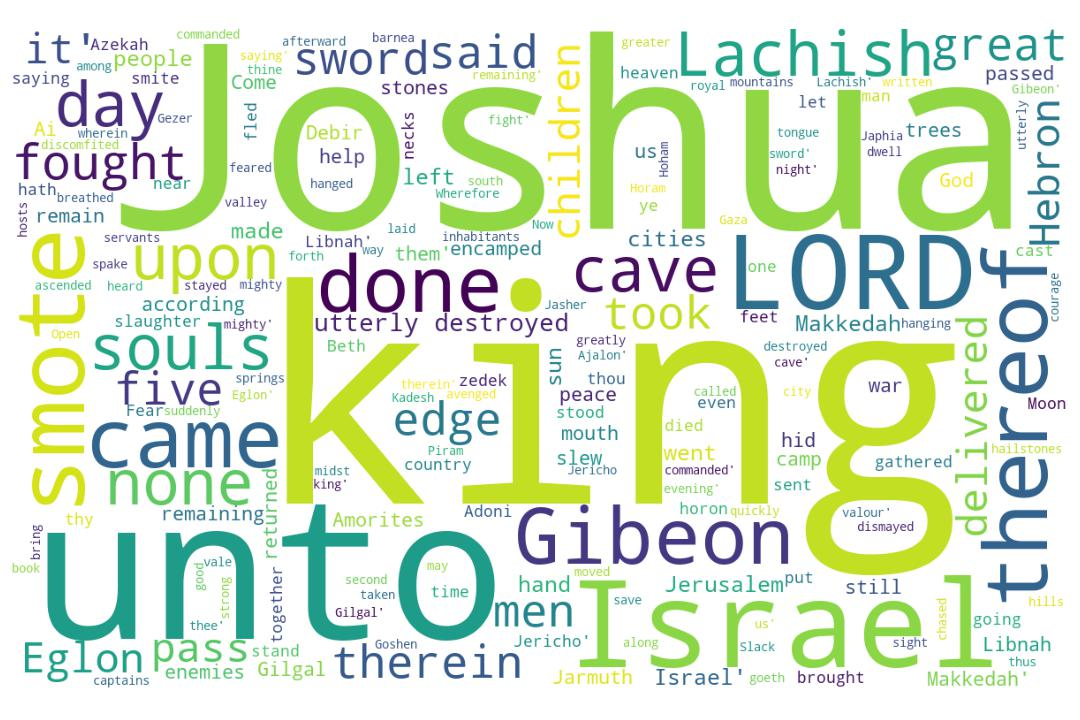
\includegraphics[width=\linewidth]{06OT-Joshua/Joshua10-WordCloud.jpg}
  \caption{Joshua 10 Word Cloud}
  \label{fig:Joshua 10 Word Cloud}
\end{figure}

\marginpar{\scriptsize \centering \fcolorbox{bone}{lime}{\textbf{THE SOUTHERN CAMPAIGN}}\\ (Joshua 10:1-43) \begin{compactenum}[I.][8]
	\item A \textbf{Strategic Advantage} \index[scripture]{Joshua!Jsh 10:01}  (Jsh 10:1) 
	\item \textbf{Solidarity} of the 5 enemy kings \index[scripture]{Joshua!Jsh 10:05}  (Jsh 10:5) 
	\item A \textbf{Surprise Attack} \index[scripture]{Joshua!Jsh 10:09}  (Jsh 10:9) 
	\item A \textbf{Slaughter} at Gibeon\index[scripture]{Joshua!Jsh 10:10}  (Jsh 10:10) 
	\item A \textbf{Stones} from heaven \index[scripture]{Joshua!Jsh 10:11}  (Jsh 10:11) 
	\item The \textbf{Stopping of the Sun} \index[scripture]{Joshua!Jsh 10:12--12}  (Jsh 10:12--13) 
	\item \textbf{Sealed} in a Cave \index[scripture]{Joshua!Jsh 10:18}  (Jsh 10:18) 
\end{compactenum}}



\footnote{\textcolor[cmyk]{0.99998,1,0,0}{\hyperlink{TOC}{Return to end of Table of Contents.}}}\footnote{\href{https://audiobible.com/bible/joshua_10.html}{\textcolor[cmyk]{0.99998,1,0,0}{Joshua 10 Audio}}}\textcolor[cmyk]{0.99998,1,0,0}{Now it came to pass, when Adoni-zedek king of Jerusalem had heard how Joshua had taken Ai, and had utterly destroyed it; as he had done to Jericho and her king, so he had done to Ai and her king; and how the inhabitants of Gibeon had made peace with Israel, and were among them;}
[2] \textcolor[cmyk]{0.99998,1,0,0}{That they feared greatly, because Gibeon \emph{was} a great city, as one of the royal cities, and because it \emph{was} greater than Ai, and all the men thereof \emph{were} mighty.}
[3] \textcolor[cmyk]{0.99998,1,0,0}{Wherefore Adoni-zedek king of Jerusalem sent unto Hoham king of Hebron, and unto Piram king of Jarmuth, and unto Japhia king of Lachish, and unto Debir king of Eglon, saying,}
[4] \textcolor[cmyk]{0.99998,1,0,0}{Come up unto me, and help me, that we may smite Gibeon: for it hath made peace with Joshua and with the children of Israel.}
[5] \textcolor[cmyk]{0.99998,1,0,0}{Therefore the five kings of the Amorites, \fcolorbox{bone}{bone}{the king of} Jerusalem, \fcolorbox{bone}{bone}{the king of} Hebron, \fcolorbox{bone}{bone}{the king of} Jarmuth, \fcolorbox{bone}{bone}{the king of} Lachish, \fcolorbox{bone}{bone}{the king of} Eglon, gathered themselves together, and went up, they and all their hosts, and encamped before Gibeon, and made war against it.}\\
\\
\P \textcolor[cmyk]{0.99998,1,0,0}{And the men of Gibeon sent unto Joshua to the camp to Gilgal, saying, Slack not thy hand from thy servants; come up to us quickly, and save us, and help us: for all the kings of the Amorites that dwell in the mountains are gathered together against us.}
[7] \textcolor[cmyk]{0.99998,1,0,0}{So Joshua ascended from Gilgal, he, and all the people of war with him, and all the mighty men of valour.}\\
\\
\P \textcolor[cmyk]{0.99998,1,0,0}{And the \fcolorbox{bone}{bone}{LORD} said unto Joshua, Fear them not: for I have delivered them into thine hand; there shall not a man of them stand before thee.}
[9] \textcolor[cmyk]{0.99998,1,0,0}{Joshua therefore came unto them suddenly, \emph{and} went up from Gilgal all night.}
[10] \textcolor[cmyk]{0.99998,1,0,0}{And the \fcolorbox{bone}{bone}{LORD} discomfited them before Israel, and slew them with a great slaughter at Gibeon, and chased them along the way that goeth up to Beth-horon, and smote them to Azekah, and unto Makkedah.}
[11] \textcolor[cmyk]{0.99998,1,0,0}{And it came to pass, as they fled from before Israel, \emph{and} were in the going down to Beth-horon, that the \fcolorbox{bone}{bone}{LORD} cast down great stones from heaven upon them unto Azekah, and they died: \emph{they} \emph{were} more which died with hailstones than \emph{they} whom the children of Israel slew with the sword.}\\
\\
\P \textcolor[cmyk]{0.99998,1,0,0}{Then spake Joshua to the \fcolorbox{bone}{bone}{LORD} in the day when the \fcolorbox{bone}{bone}{LORD} delivered up the Amorites before the children of Israel, and he said in the sight of Israel, Sun, stand thou still upon Gibeon; and thou, Moon, in the valley of Ajalon.}
[13] \textcolor[cmyk]{0.99998,1,0,0}{And the sun stood still, and the moon stayed, until the people had avenged themselves upon their enemies. \emph{Is} not this written in the book of Jasher? So the sun stood still in the midst of heaven, and hasted not to go down about a whole day.}
[14] \textcolor[cmyk]{0.99998,1,0,0}{And there was no day like that before it or after it, that the \fcolorbox{bone}{bone}{LORD} hearkened unto the voice of a man: for the \fcolorbox{bone}{bone}{LORD} fought for Israel.}\\
\\
\P \textcolor[cmyk]{0.99998,1,0,0}{And Joshua returned, and all Israel with him, unto the camp to Gilgal.}
[16] \textcolor[cmyk]{0.99998,1,0,0}{But these five kings fled, and hid themselves in a cave at Makkedah.}
[17] \textcolor[cmyk]{0.99998,1,0,0}{And it was told Joshua, saying, The five kings are found hid in a cave at Makkedah.}
[18] \textcolor[cmyk]{0.99998,1,0,0}{And Joshua said, Roll great stones upon the mouth of the cave, and set men by it for to keep them:}
[19] \textcolor[cmyk]{0.99998,1,0,0}{And stay ye not, \emph{but} pursue after your enemies, and smite the hindmost of them; suffer them not to enter into their cities: for the \fcolorbox{bone}{bone}{LORD} your God hath delivered them into your hand.}
[20] \textcolor[cmyk]{0.99998,1,0,0}{And it came to pass, when Joshua and the children of Israel had made an end of slaying them with a very great slaughter, till they were consumed, that the rest \emph{which} remained of them entered into fenced cities.}
[21] \textcolor[cmyk]{0.99998,1,0,0}{And all the people returned to the camp to Joshua at Makkedah in peace: none moved his tongue against any of the children of Israel.}
[22] \textcolor[cmyk]{0.99998,1,0,0}{Then said Joshua, Open the mouth of the cave, and bring out those five kings unto me out of the cave.}
[23] \textcolor[cmyk]{0.99998,1,0,0}{And they did so, and brought forth those five kings unto him out of the cave, \fcolorbox{bone}{bone}{the king of} Jerusalem, \fcolorbox{bone}{bone}{the king of} Hebron, \fcolorbox{bone}{bone}{the king of} Jarmuth, \fcolorbox{bone}{bone}{the king of} Lachish, \emph{and} \fcolorbox{bone}{bone}{the king of} Eglon.}
[24] \textcolor[cmyk]{0.99998,1,0,0}{And it came to pass, when they brought out those kings unto Joshua, that Joshua called for all the men of Israel, and said unto the captains of the men of war which went with him, Come near, put your feet upon the necks of these kings. And they came near, and put their feet upon the necks of them.}
[25] \textcolor[cmyk]{0.99998,1,0,0}{And Joshua said unto them, Fear not, nor be dismayed, be strong and of good courage: for thus shall the \fcolorbox{bone}{bone}{LORD} do to all your enemies against whom ye fight.}
[26] \textcolor[cmyk]{0.99998,1,0,0}{And afterward Joshua smote them, and slew them, and hanged them on five trees: and they were hanging upon the trees until the evening.}
[27] \textcolor[cmyk]{0.99998,1,0,0}{And it came to pass at the time of the going down of the sun, \emph{that} Joshua commanded, and they took them down off the trees, and cast them into the cave wherein they had been hid, and laid great stones in the cave's mouth, \emph{which} \emph{remain} until this very day.}\\
\\
\P \textcolor[cmyk]{0.99998,1,0,0}{And that day Joshua took Makkedah, and smote it with the edge of the sword, and the king thereof he utterly destroyed, them, and all the souls that \emph{were} therein; he let none remain: and he did to \fcolorbox{bone}{bone}{the king of} Makkedah as he did unto \fcolorbox{bone}{bone}{the king of} Jericho.}
[29] \textcolor[cmyk]{0.99998,1,0,0}{Then Joshua passed from Makkedah, and all Israel with him, unto Libnah, and fought against Libnah:}
[30] \textcolor[cmyk]{0.99998,1,0,0}{And the \fcolorbox{bone}{bone}{LORD} delivered it also, and the king thereof, into the hand of Israel; and he smote it with the edge of the sword, and all the souls that \emph{were} therein; he let none remain in it; but did unto the king thereof as he did unto \fcolorbox{bone}{bone}{the king of} Jericho.}\\
\\
\P \textcolor[cmyk]{0.99998,1,0,0}{And Joshua passed from Libnah, and all Israel with him, unto Lachish, and encamped against it, and fought against it:}
[32] \textcolor[cmyk]{0.99998,1,0,0}{And the \fcolorbox{bone}{bone}{LORD} delivered Lachish into the hand of Israel, which took it on the second day, and smote it with the edge of the sword, and all the souls that \emph{were} therein, according to all that he had done to Libnah.}\\
\\
\P \textcolor[cmyk]{0.99998,1,0,0}{Then Horam king of Gezer came up to help Lachish; and Joshua smote him and his people, until he had left him none remaining.}\\
\\
\P \textcolor[cmyk]{0.99998,1,0,0}{And from Lachish Joshua passed unto Eglon, and all Israel with him; and they encamped against it, and fought against it:}
[35] \textcolor[cmyk]{0.99998,1,0,0}{And they took it on that day, and smote it with the edge of the sword, and all the souls that \emph{were} therein he utterly destroyed that day, according to all that he had done to Lachish.}
[36] \textcolor[cmyk]{0.99998,1,0,0}{And Joshua went up from Eglon, and all Israel with him, unto Hebron; and they fought against it:}
[37] \textcolor[cmyk]{0.99998,1,0,0}{And they took it, and smote it with the edge of the sword, and the king thereof, and all the cities thereof, and all the souls that \emph{were} therein; he left none remaining, according to all that he had done to Eglon; but destroyed it utterly, and all the souls that \emph{were} therein.}\\
\\
\P \textcolor[cmyk]{0.99998,1,0,0}{And Joshua returned, and all Israel with him, to Debir; and fought against it:}
[39] \textcolor[cmyk]{0.99998,1,0,0}{And he took it, and the king thereof, and all the cities thereof; and they smote them with the edge of the sword, and utterly destroyed all the souls that \emph{were} therein; he left none remaining: as he had done to Hebron, so he did to Debir, and to the king thereof; as he had done also to Libnah, and to her king.}\\
\\
\P \textcolor[cmyk]{0.99998,1,0,0}{So Joshua smote all the country of the hills, and of the south, and of the vale, and of the springs, and all their kings: he left none remaining, but utterly destroyed all that breathed, as the \fcolorbox{bone}{bone}{LORD} God of Israel commanded.}
[41] \textcolor[cmyk]{0.99998,1,0,0}{And Joshua smote them from Kadesh-barnea even unto Gaza, and all the country of Goshen, even unto Gibeon.}
[42] \textcolor[cmyk]{0.99998,1,0,0}{And all these kings and their land did Joshua take at one time, because the \fcolorbox{bone}{bone}{LORD} God of Israel fought for Israel.}
[43] \textcolor[cmyk]{0.99998,1,0,0}{And Joshua returned, and all Israel with him, unto the camp to Gilgal.}
